\chapter {State of the Art}

\section{\gls{eeg}}
\gls{eeg} is a non-invasive method for measuring and recording electrical brain activity along the scalp. This measurement is based on registering voltage changes from the brain neurons using electrodes, which are attached on a scalp. The \gls{erp} technique allows us to take raw \gls{eeg} data, the electrical activity recorded from the brain, and use it to investigate cognitive processing. It is recorded a subject's \gls{eeg} while they perform a task designed to elicit the proper cognitive response (e.g. attending to a certain type of object). To accomplish this subjects wear a mesh cap embedded with electrodes which record brain activity. \cite{erpinfo} The position and designation of electrodes is defined in the international system 10-20 (Figure~\ref{10-20}), but the scheme was extended and now defines positions for 70 electrodes. Signals from electrodes are recorded and then analyzed. The research of driver's attention, children's motor coordination disorder or mouse blindness is ongoing at University od West Bohemia. \gls{eeg} measurement is not focused only on humans, but is conducted also on animals or cells. Brain activity from electrodes is recorded during measurements, and for \gls{erp} experiments, stimuli are also recorded. Stimuli are synchronized with \gls{eeg} recording to determine subjects' responses.

Each year, an increasingly vast amount of neuroscience electrophysiology data is collected and reported in journal publications. However, almost none of these data are accessible to the community of theorists building integrative models of neuronal systems or to experimentalists planning new experiments. \cite{incf_mission}

\begin{SCfigure}
	\centering
	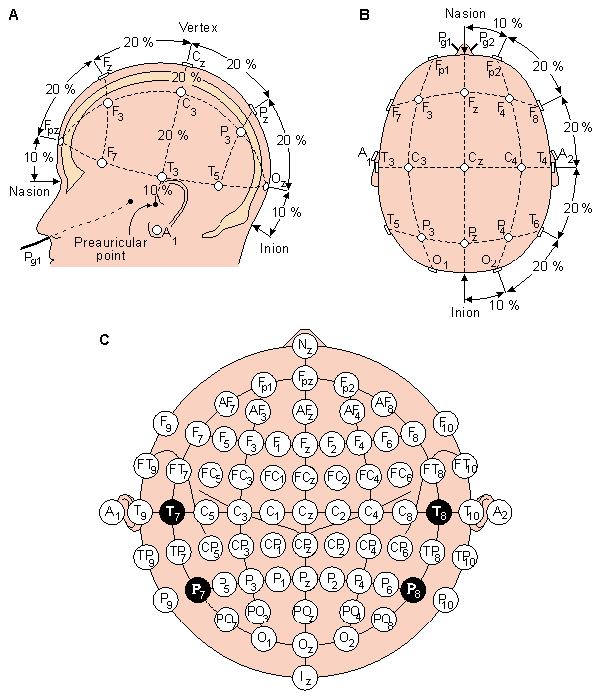
\includegraphics[scale=0.4]{obrazky/ElectrodePositions1020.png}
	\caption{The original 10-20 international system - internationally recognized method to describe and apply the location of scalp electrodes in the context of an EEG test or experiment. \cite{BCI2000}}
	\label{10-20}
\end{SCfigure}

\section{Data Sharing}

A trend toward increased sharing of neuroimaging data has emerged in recent years. Nevertheless, a number of barriers continue to impede easy sharing of experiment's data. Many researchers and institutions remain uncertain about how to share data or lack the tools and expertise to participate in data sharing. The use of \gls{edc} (Figure~\ref{stages-edc}) methods for neuroimaging greatly simplifies the task of data collection and has the potential to help standardize many aspects of data sharing. \cite{neuroinf} The motivation for sharing is:
\begin{itemize}
	\item \textbf{to accelerate progress in understanding of the brain}
	
	
	Several researchers claim that more rapid scientific discoveries are possible with shared data \cite{Milham2012} \cite{Poldrack2012}.
	\item \textbf{to improve data quality}
	
	The sharing data helps uncover mistakes as missing data, noise, errors, etc. and improves the quality of the data in the future experiments.
	\item  \textbf{to reduce cost of research} 
	
	Neuroimaging research is costly both in terms of the data acquisition costs and the time spent in data documentation. A significant amount of money could be saved from redundant data acquisition if data were shared with appropriate metadata descriptions. \cite{neuroinf}
\end{itemize} 

The situation is similar in electroencephalography. \cite{neuroinf} \cite{mrieeg}  \cite{incf_mission}


\begin{figure}
	\centering
	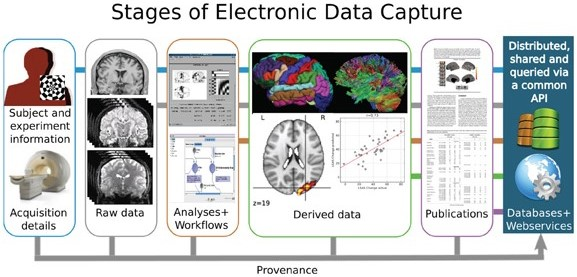
\includegraphics[scale=0.6]{obrazky/stages-EDC.jpg}
	\caption {Stages of Electronic Data Capture. \cite{neuroinf}}
	\label{stages-edc}
\end{figure}


\section{Program on Standards for Data Sharing}
\label{incf}
\gls{incf} Program on Standards for Data Sharing was established for the purpose of specification the standard for storing \gls{eeg} data. \gls{incf} is an international non-profit organization devoted to advancing the field of neuroinformatics and was established in 2005 in Stockholm. \gls{incf} community consists of 17 member countries and associated research groups, consortia, funding agencies and publishers in the field. The National Nodes are institutions or networks that represent each member country. The nodes are established to coordinate neuroinformatics activity within a country.  \cite{incfweb}

Program Standards for Data Sharing aims to develop generic standard and tools to facilitate the recording, sharing, and reporting of neuroscience metadata in order to improve practices for the archiving and sharing of neuroscience data. Metadata define the methods and conditions of data acquisition and subsequent analytical processing, Metadata also describe conditions under which the actual raw-data were acquired.

The current focus of the Program on Standards for Data Sharing is in two areas: neuroimaging and electrophysiology. \cite{incf_mission}. The most important requirement of such a standard is to accommodate common types of data used in electrophysiology or neuroimaging and also the metadata required to describe them. However we will focus on electrophysiology.

A standard way of storing metadata must be specified. The set of metadata required to describe electrophysiology data is difficult to determine a priori because the types of experiments are so varied.  A flexible mechanism must be used which allows referencing and specifying values for currently existing ontologies and also accommodates information not currently systematized. Techniques to include post-experiment annotations of data, and for relating different data parts, are also required. \cite{hdf5standard}

So far, the working group entertains two approaches towards defining a standard, which may eventually be merged. One, currently named Pandora, defines a generic data model that can be used with \gls{hdf5} or other storage back-ends. Due to the generic nature, the data model can be used to store various kinds of neuroscience data. The other proposal, called epHDF, defines domain specific schemata for storing electrophysiology data in \gls{hdf5}. \cite{hdf5standard}

The Electrophysiology Task Force of the \gls{incf} Program on Standards for Data Sharing is working on a document Requirements for storing electrophysiology data. The last version is 0.72 from 3rd November, 2014. This \gls{incf} internal document specifies all data that the standardized file format requires, defining what it must, should and may support. An overview of the stored data types is in Table~\ref{data_types}. \cite{requirements}
\begin{table}
	\begin{center}
		\begin{tabular}{|c|p{9cm}|}
			\hline Data type  & Description \\ 
			\hline Signal source & The origin of the recorded data; for example, the identity, position, etc. of the recording. This typically refers to information about a channel name, description, and location, or the target recorded.  There are at least two kinds of sources, including actors doing the recording (e.g. an electrode) and objects/actors being recorded (e.g. an subject, brain region, or neuron (real or putative))   \\ 
			\hline  Time series & An ordered collection of values given at defined points in time; for example, a recorded voltage  signal. It may correspond to raw data, recorded from “electrodes” or “channels”.   Alternatively, they could be derived from a data processing step.  The sampling may be done at regular time intervals (the sampling rate) or at irregular intervals (in which case a time point is required for each value).   \\ 
			\hline Signal events & The Signal events identify changes in a signal; for example, spikes, synaptic potentials, artifacts.  They could be raw data, for example, output of a hardware device that detects, and provides the times of spikes. They may also be generated as the result of processing data, for example, applying a spike detection algorithm on a time series signal. \\ 
			\hline  Image stacks & Image stacks are an ordered collection of images; the meaning of stack dimensions must be specified.  For example, a z-stack of images, a time series of images, a time-series of z-stacks, movies which are in standard formats.   \\ 
			\hline Experimental events & The Experimental Events data type consists of times of events, along with values that correspond to the times.   This data type can be used to describe: stimuli, trials or sweeps, time intervals, behaviors, and other events or conditions that occur during the experiment.   \\ 
			\hline Other / Generic array & Other data types and a mechanism for storing data types which have not been included in the standard. \\ 
			\hline 
		\end{tabular} 
		
		\caption{Overview of data types required by Requirements for storing electrophysiology data, Version 0.72. \cite{requirements}}
		\label{data_types}
	\end{center}
\end{table}






\section{Present formats for Storing \gls{eeg} Data}
Most known formats for storing \gls{eeg} data use the format \gls{hdf5}. Also both \gls{incf} proposals use \gls{hdf5} and the Electrophysiology Task Force of the INCF Program on Standards for Data Sharing in Requirements for a standard recommends basing a standard on \gls{hdf5}. \cite{requirements} Some formats are proprietary and even though some of them are well documented, is due to licenses complicated to use them or edit them. So I focus on the open ones. For storing \gls{eeg} neuroinformatics data many types of formats exist. The most known and used formats are Ovation \cite{ovation}, NeXus Format \cite{nexus}, NEO \cite{neo}, NeuroHDF \cite{neurohdf}, EDF+ \cite{kemp2003} and NIX (Pandora) \cite{pandora}. 

\subsection{Ovation}
Ovation is a commercial system for managing laboratory scientific data. The Ovation natively stores data in a database, but the data can be exported in \gls{hdf5} container. Ovation is cloud based data management and collaboration portal. It organizes files by projects and experiments while maintaining relationships between files and subjects, devices, and protocols used in experiment. \cite{ovation2} The description of the work model of Ovation is in Figure~\ref{ovation_work}. Although Ovation is a commercial system, the data model of Ovation is open \cite{ovation_m}. 

\begin{figure}
	\begin{center}
		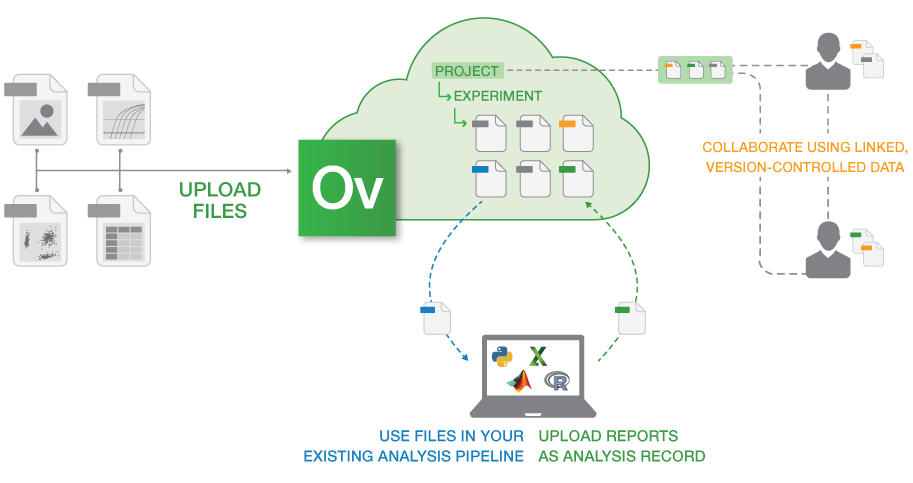
\includegraphics[scale=0.43]{obrazky/ovation.png}
		\caption{Ovation work model - Researchers upload their data into Ovation portal and describe them. Then they could work with data with existing analyze tools or work directly with project with linked version-controlled data. \cite{ovation2}}
		\label{ovation_work}
	\end{center}
\end{figure}

\subsection{European Data Format}
\gls{edf} is a format for storing multichannel biological and physical signals. This format has limitations for application in a field of evoked potentials, cardiology etc. A major limitation is that \gls{edf} can store only uninterrupted recordings. \gls{edf}+ was specified for that reasons. The EDF+ specification is incompatible with \gls{edf} only in allowing storage of several non-contiguous recordings. The \gls{edf} format support annotation for text, event and stimuli. An EDF and EDF+ data file consists of a header record followed by data records. The variable-length header record identifies the patient and specifies the technical characteristics of the recorded signals. \cite{edf} Information about signals, subject and whole measurements is defined and could not be changed. EDF+ format contains this information: version of format, patient identification (sex, birth date, subjects name), record identification (start date, start time, hardware identification, a code specifying the responsible investigator, a code specifying used equipment), number of data records, duration of records and number of signals in data record.


\subsection{NeXus Format}
\label{nexus_format}
NeXus is a format for data from Neutron and X-ray facilities. The format is also used for muon experiments. NeXus uses \gls{hdf5} as a default file container, but for compatibility reasons it is possible to use also \gls{hdf4} or \gls{xml} for special use cases. This format supports saving data and metadata into a single file. Several schemes are available for storing metadata sections, but the terminology is not defined and informations are stored in general structures as note, log, parameter or characterization. \cite{nexus}

\subsection{NEO}
Neo is a package for representing electrophysiology data in Python. This software package is able to load data from closed manufacturers' formats as Axon, Spike2, AlphaOmega, BlackRock and others. Neo implements a hierarchical data model and supports exporting to several neutral formats including \gls{hdf5}, MATLAB .mat file with NEO structure (NeoHDF5, NeoMatlab,.. ) or other open source tools WinEdr, WinWcp, PyNN, etc. The recommended way of use of this package is converting a closed format into more standard and open formats - NeoHDF5 or NeoMatlab. 



The goal of Neo is to improve interoperability between Python tools for analyzing, visualizing and generating electrophysiology data by providing a common, shared object model. In order to be as lightweight a dependency as possible, Neo is deliberately limited to presentation of data, with no functions for data analysis or visualization. Neo implements a hierarchical data model well adapted to intracellular and extracellular electrophysiology and \gls{eeg} data with support for multi-electrodes. \cite{neo}

\subsection{NeuroHDF}
This format also uses \gls{hdf5} as the main container for storing data. NeuroHDF is an effort to combine the flexibility and efficiency of \gls{hdf5} for neuroscience datasets through the specification of a simple layout for different data types with minimal metadata. \cite{neurohdf} 

\subsection{NIX}
\label{nixsection}
This format also uses \gls{hdf5} as a data container. This format specification closely defines an inner structure of file, especially the data part. The meta data part is defined by the \gls{odml}. 
The NIX project (previously called Pandora) started in the context of the Electrophysiology Task Force which is part of the \gls{incf} Datasharing Program. 

NIX is one approach to this problem: it uses highly generic models for data as well as for metadata and defines standard schemata for \gls{hdf5} files representing these models. Last but not least NIX aims to provide a convenient C++ library to simplify the access to the defined format. The design principle of the data model used by NIX was to create a rather minimalistic, generic, yet expressive model that is able to represent data stored in other widely used formats or models like Neuroshare or NEO without any loss of information. Due to its generic approach, the data model is also able to represent other kinds of data used in the field e.g. image data or image stacks. \cite{pandora}

\begin{figure}
	\begin{center}
		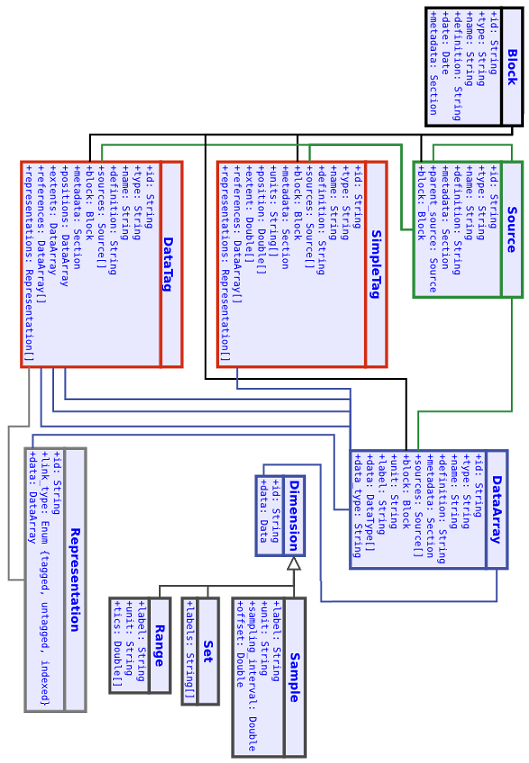
\includegraphics[scale=0.95]{obrazky/NIX_scheme.png}
		\caption{NIX data scheme. \cite{pandora}}
		\label{NIX_scheme}
	\end{center}
\end{figure}

This format's scheme (Figure~\ref{NIX_scheme}) was taken as inspiration for my file format, because it is discussed within the INCF Datasharing Program (Chapter~\ref{incf}) and it is recommended to use the file model of NIX. The measurements are stored in blocks. Each block identifies measurement and related metadata section. Raw data (signals, stimuli) are saved in DataArrays and they are specified by Dimension, Sample, Set, Representation and Range (Figure~\ref{NIX_scheme}) and could be specified by DataTag. The stimuli and artifacts are stored in SimpleTag (one stimulus) or MultiTag (more stimuli). The source of DataArrays or Tags could be specified by Source. Each section could contain link to the metadata part with measurement information. Closer description is available in Section~\ref{section_data}.



\subsection{epHDF}
This format is discussed within the \gls{incf} Program on Data Sharing standard. It uses \gls{hdf5} and deals with two issues. It is virtually impossible to anticipate all of the types of data and metadata that will need to be stored and no standard scheme exists for specifying how data in \gls{hdf5} files should be organized. \cite{ephdf}
To address both of these difficulties, a layered approach is proposed.  The first layer, which is called \gls{hdfds}, provides domain-independent conventions for specifying how the data in \gls{hdf5} files are organized. 
 Main features of \gls{hdfds} are as follows: 
\begin{itemize}
\item Enables associating external schemata to components of an \gls{hdf5} file in a manner similar to how name spaces in an XML file identify elements. 
\item Specifies locations and a format for storing arbitrary metadata in a \gls{hdf5} file. 
 \item Allows linking metadata to particular data parts within a file and to external files. \cite{ephdf}
\end{itemize}

The second layer builds on the conventions in \gls{hdfds} to specify schemata for storing basic electrophysiology data types.  It is called second layer \gls{ephdf}.  The data types defined in \gls{ephdf} (time series, time series segment, neural event and experimental event) are based on the entities defined in Neuroshare \cite{neuroshare} for covering the most commonly used data types in electrophysiology.  For each type, the data can be stored in whatever \gls{hdf5} numeric format is most efficient (for example 16 bit integer).  For all of the data types, a metadata schema is specified to include the fields needed to make a plot of the data with correct units. \cite{ephdf}

The epHDF for storing metadata uses \gls{odml}. An example of data annotation using \gls{odml} and \gls{json} encoding is bellow in listing~\ref{ephdf_example}. The listing shows description of amplifier hardware and its parameters. \cite{ephdf}
\newpage

\begin{lstlisting}[language=XML,label=ephdf_example,caption=Example of  data annotation using odML and JSON encoding.]
{
  "schema": "odml:hardware/amplifier.xml",
  "model" : <string_value>,
  "manufacture" : <string_value>,
  "serial_no" : <string_value>,
  "inventory_no": <string_value>,
  "owner" : <string_value>,
  "amplifier_type": <string_value>,
  "measurement_type": <string_value>,
  "operation_mode": <string_value>,
  "switching_frequence": <numeric_value>,
  "duty_cycle" : <numeric_value>,
  "gain" : <numeric_value>,
  "high_pass_cutoff" : <numeric_value>,
  "low_pass_cutoff" : <numeric_value>,
}
\end{lstlisting} 

\subsection{Brain Vision Format}

\gls{eeg} data at \gls{uwb} are recorded by BrainVision Recorder \cite{brainvision} (Figure~\ref{recorder}). This program records raw data and saves it to three files, which are described in the next chapter. 

The BrainVision Recorder does not allow natively recorded data in any other format. Most recordings consist of three files. The format of these files is defined in the BrainVision Recorder User Manual \cite{brainUserManual}:
\begin{itemize}
	\item \textbf{data file}
	\label{eeg}
	
	This is binary file which contains recorded values from recording device. The data are stored as double numbers.
	
	\item \textbf{vhdr file}
	\label{vhdr}
	
	This text file is Brain Vision Data Exchange Header File Version 1.0 and includes basic information about measurements. The format of the header file is based on the Windows INI format. It consists of various named sections containing keywords/values. The file stores basic information about measuring: coding, name of data file, name of marker file, number of channels, sampling interval in microseconds, information about binary format (IEEE\_FLOAT\_32) and information about channels (Channel number, channel name, resolution of unit, unit). The sample file of stored data and metadata is in listings~\ref{HeaderFile1} ~\ref{HeaderFile2} ~\ref{HeaderFile3} ~\ref{HeaderFile5} and table~\ref{HeaderFile4}. The sample file shows data saved in the EEGBase format.
	
	\item \textbf{vmrk file}
	\label{vmrk}
	
	This is Brain Vision Data Exchange Marker File, Version 1.0. The marker file is based upon the same principle of sections and keywords as the header file. This text file contains information about markers. The file stores marker number, type of the marker, description, position, size and channel number. The example of file is in Listing~\ref{vmrk_file}.
	
\end{itemize}


\lstset{aboveskip=3mm,
	belowskip=3mm,
	showstringspaces=false,
	columns=flexible,
	basicstyle={\small\ttfamily},
	breaklines=true,
	breakatwhitespace=true,
	tabsize=3,
	mathescape
}


\begin{lstlisting}[frame=single,caption={The header file example - Information about the file format.},label=HeaderFile1]
Brain Vision Data Exchange Header File Version 1.0
; Data created by the Vision Recorder
\end{lstlisting}
\begin{lstlisting}[frame=single,caption={The header file example - Information about coding, created files, data orientation, number of recorded channels and sampling interval.},label=HeaderFile2]
[Common Infos]
Codepage=UTF-8
DataFile=000007.eeg
MarkerFile=000007.vmrk
DataFormat=BINARY
; Data orientation: MULTIPLEXED=ch1,pt1, ch2,pt1 ...
DataOrientation=MULTIPLEXED
NumberOfChannels=48
; Sampling interval in microseconds
SamplingInterval=5000
\end{lstlisting}







\begin{SCfigure}[][h]
	\caption{Software used for EEG recording at University of West Bohemia - BrainVision Recorder. \cite{brainvision}}
	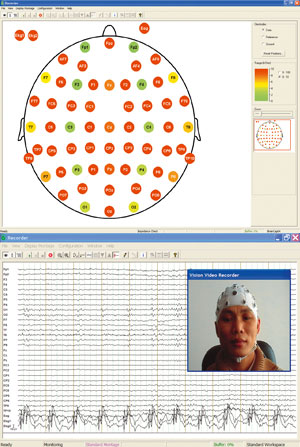
\includegraphics{obrazky/recorder.png}	
	\label{recorder}
\end{SCfigure}

\section{Hierarchical Data Format}

\gls{hdf} is a data model, file format and library for storing extremely large and complex data collections. \cite{hdf} This technology is able to store any kind of data and is used all over the world in research centers and government agencies. For example the format \gls{hdf5} is used by Cardiff University for resolving their problem with grid computing, Deutsche Bank for financial engineering, Diamond Light Source in synchrotron science (using NeXus format- Section \ref{nexus_format}), Laboratory for Neural Computation for bio-engineering and many others. A lot of formats for storing electrophysiology data use \gls{hdf5}. The adopters are able to solve variety of problems with \gls{hdf} format. (Figure~\ref{hdf_why}). 
"The grouping structure in \gls{hdf5} enables applications to organize data objects in \gls{hdf5} to reflect complex relationships among objects. The rich collection of \gls{hdf5} datatypes, including datatypes that can point to data in other objects, and including the ability for users to define their own types, lets applications build sophisticated structures that match well with complex data. The \gls{hdf5} library has a correspondingly rich set of operations that enables applications to access just those components that are important." \cite{hdf}


\gls{hdf} is similar to \gls{xml} documents, \gls{hdf} files allows to specify complex data relationships and dependencies and are self-describing. Several APIs for programing languages C, C++, Fortran 90, Java and others are available for this format. 
\gls{hdf} is open-source (\gls{bsd} license), stored data are human readable and the metadata model is easily customized.


\begin{figure}[h]
	\begin{center}
		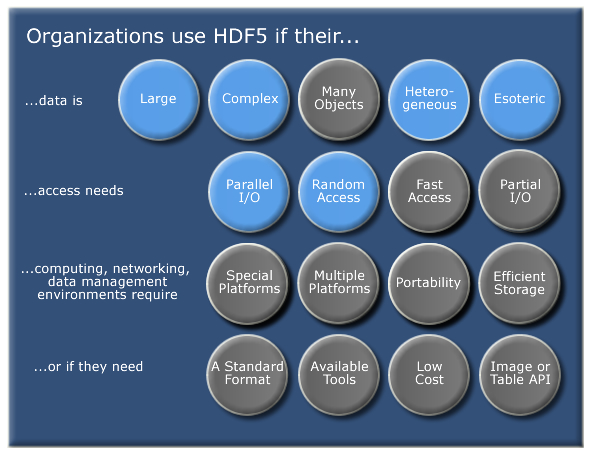
\includegraphics[scale=0.85]{obrazky/hdf_why.png}
		\caption{Detailed descriptions of some of the data challenges facing HDF adopters. \cite{hdf}}
		\label{hdf_why}
	\end{center}
\end{figure}

The advantages of using \gls{hdf5}: \cite{neurohdf}
\begin{itemize}
	\item \textbf{Compact binary data storage, extensible metadata}
	
	The \gls{hdf5} container could use software lossless compression. Szip and Gzip are a stand-alone libraries that are configured as optional filters in \gls{hdf5}. An Application is using Szip or Gzip compression when a dataset is created and if Szip (Gzip) encoder is enabled, data is automatically compressed and decompressed by Szip (an implementation of the extended-Rice lossless compression algorithm) or Gzip compression. (Figure~\ref{hdf_compression}). \gls{hdf5} allows to use third party compression filters too.
	
	
	\begin{SCfigure}
		\centering
			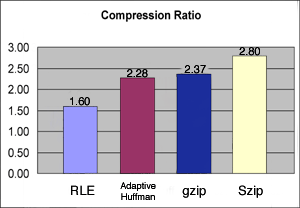
\includegraphics[scale=0.89]{obrazky/H4_szip_size.png}
			\caption{Comparison of compression performance in tests with HDF4. Size of compressed output with Szip in HDF4. The test were conducted with HDF4 format, but the compression algorithms are the same in HDF5.}
			\label{hdf_compression}
	\end{SCfigure}
	
	\item \textbf{Fast random and parallel access, efficient, scalable}
	
	The \gls{hdf} already supports parallel I/O and there is project of the European synchrotron particle accelerator community on developing the capability for multiple reader processes to read from an HDF5 file while another process writes to the file. The \gls{hdf} container supports compression.
	\item \textbf{Widely used in High Performance Computing}
		
	\item \textbf{Open source and cross-platform}
	
	The \gls{hdf5} format is open source and the HDF Group offers API in many languages (C, Java, Python, Fortran,..) for a various platforms.
	\item \textbf{Possible speed up the query} \cite{hdffast}
\end{itemize}
Possible limitations of \gls{hdf5}: \cite{neurohdf}
\begin{itemize}
	\item \textbf{Difficulty to store variable-length string properties.}
	
	Storing of string properties is not simple, especially for strings with variable length.
	\item \textbf{Deleting a dataset does not free the space on disk.}
	
	The deletion of a dataset from \gls{hdf5} file does not free the space and the dataset stays in the file (but is inaccessible). The release of the space on disk requires rewriting the file.

	\item \textbf{Evaluating \gls{hdf5}}
	
	There is no tool to evaluate \gls{hdf5} files. The \gls{hdf} allows storing of any data and it is complicated to evaluate it.
	\item \textbf{Delete or update a dataset in \gls{hdf5}} 
	
	The size of the dataset cannot be reduced after it is created. The dataset can be expanded by extending one or more dimensions, with function H5Dextend. It is not possible to contract a dataspace, or to reclaim allocated space.
\end{itemize}

\section{Ontologies}

Ontologies are formalized vocabularies of terms. Yann Le Franc defined ontologies this way: "Ontologies are formal models of knowledge in a particular domain and composed of classes that represent concepts defining the field as well as the logical relations that link these concepts together." \cite{ontology} The model of ontology is in Figure~\ref{ontology_scheme}.

\begin{SCfigure}[][h]
	\centering
	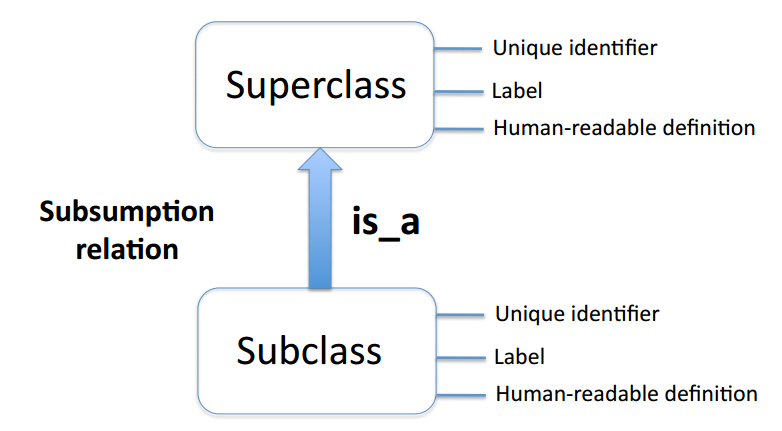
\includegraphics[scale=0.5]{obrazky/ontology.png}
	\caption{Ontology model. \cite{ontology}}
	\label{ontology_scheme}
\end{SCfigure}

\subsection{Neural ElectroMagnetic Ontology}
Neural ElectroMagnetic Ontology describes classes of event-related brain potentials and their properties, including spatial, temporal, and functional (cognitive/behavioral) attributes, and data-level attributes (acquisition and analysis parameters). \cite{nemo}
\subsection{Gene Ontology}
This project provides an ontology of defined terms representing gene product properties. 
The ontology covers three domains: cellular component, molecular function and biological process. \cite{bruha}
\subsection{Phenotype And Trait Ontology}
"Phenotype And Trait Ontology is an ontology of phenotypic qualities intended for use in a number of applications, primarily defining composite phenotypes and phenotype annotation, Phenotypic qualities (properties). This ontology can be used in conjunction with other ontologies." \cite{bruha}
\subsection{The Open Biomedical Ontologies Foundry}
The \gls{obo} Foundry is a collaborative experiment involving developers of science-based ontologies who are establishing a set of principles for ontology development with the goal of creating a suite of orthogonal interoperable reference ontologies in the biomedical domain. \cite{oen}
\subsection{OBO Relations Ontology}
Relations Ontology is a collection of relations intended primarily for standardization across ontologies in the \gls{obo} Foundry and wider \gls{obo} library. It incorporates core upper-level relations such as part of as well as biology-specific relationship types such as develops form. \cite{smith2005}
\subsection{NIFSTD}
\gls{nifstd} is a core component of \gls{nif} project, a semantically enhanced portal for accessing and integrating neuroscience data, tools and information. \gls{nifstd} includes a set of modular ontologies that provide a comprehensive collection of terminologies to describe neuroscience data and resources. \cite{nifstd}
\subsection{Basic Formal Ontology}
The \gls{bfo} is a small, upper level ontology that is designed for use in supporting information retrieval, analysis and integration in scientific and other domains. \gls{bfo} is a genuine upper ontology designed to serve data integration in scientific and other domains. Thus it does not contain physical, chemical, biological or other terms which would properly fall within the coverage domains of the special sciences.  \cite{bfo}
\subsection{Computational Neuroscience Ontology}
\gls{cno} is a controlled vocabulary of terms used in Computational Neurosciences to describe models of the nervous system. This first release of \gls{cno} is an alpha version and should be further aligned with other ontologies accessible on Bioportal and should be made compliant with the \gls{obo} foundry recommendations. \cite{cno}
\subsection{Ontology for Biomedical Investigations}
Ontology for Biomedical Investigations is an ontology of investigations, the protocols and instrumentation used, the material used, the data generated and the types of analysis performed on it. \cite{obi}


\section{Open Metadata Markup Language}

\begin{figure}[h]
	\begin{center}
		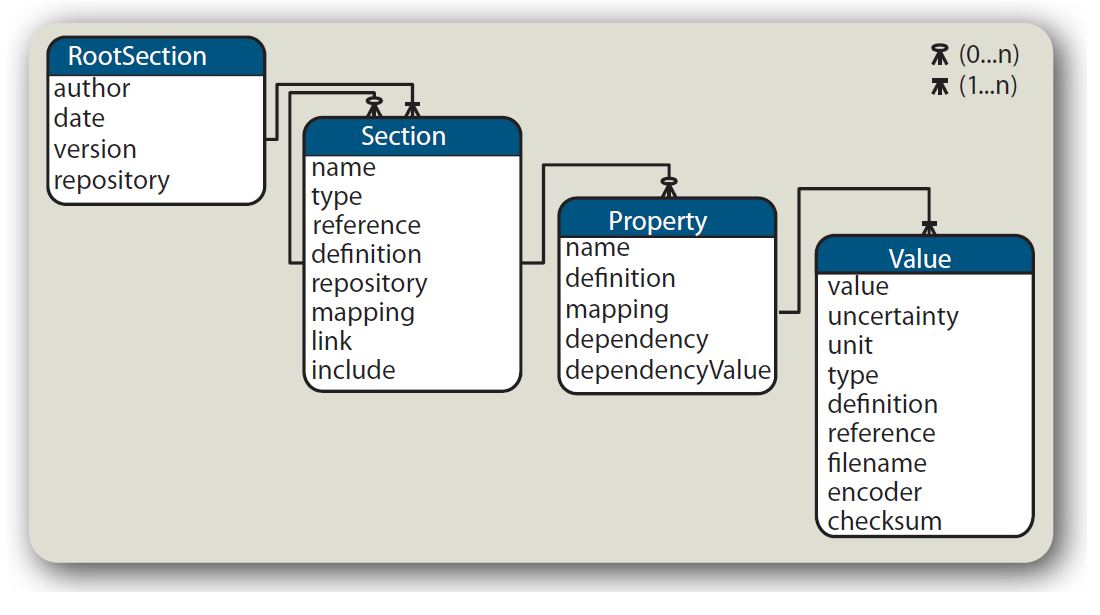
\includegraphics[scale=0.4]{obrazky/odml_tree.jpg}
		\caption{Open metadata Markup Language Entity-Relation diagram. \cite{odml}}
		\label{odml-tree}
	\end{center}
\end{figure}	
The metadata in electrophysiology domain providing information about stimuli, data acquisition, and experimental conditions are indispensable for the analysis and the management of experimental data within a lab. However, only rarely are metadata available in a structured, comprehensive, and machine-readable form. This poses a severe problem for finding and retrieving data, both in the laboratory and on the various emerging public data bases. \cite{odml} The \gls{odml} defines the format, not the content, so that it is inherently extensible and can be adapted to the specific requirements of any laboratory. For data sharing a correct understanding of metadata and data is only possible if the same terminology is used or if mappings between terminologies are provided. For this purpose were assembled terminologies with definitions of commonly used terms. \cite{odmlarticle}


\lstset{aboveskip=3mm,
	belowskip=3mm,
	showstringspaces=false,
	columns=flexible,
	basicstyle={\small\ttfamily},
	breaklines=true,
	breakatwhitespace=true,
	tabsize=3,
	mathescape
}
\begin{lstlisting}[language=xml,frame=single,label=odml_example,caption=Example of odml XML file.]
<?xml version="1.0" encoding="ISO-8859-1"?>
<?xml-stylesheet type="text/xsl" href="odmlTerms.xsl"  xmlns:odml="http://www.g-node.org/odml"?>
<!-- ********************************************************* -->
<!--                     Subject section                       -->
<!-- ********************************************************* -->
<odML version="1">
<repository>
http://portal.g-node.org/odml/terminologies/v1.0/terminologies.xml
</repository>
<version>1.0</version>
<date>2011-01-21</date>
<section>
<type>subject</type>
<name>Subject</name>
<definition>The investigated experimental subject (animal or person). May contain the Cell and Preparation sections as subsections.</definition>

<property>
<name>Comment</name>
<value>
<type>text</type>
</value>
<definition>A general comment on a specific subject. </definition>
</property>
\end{lstlisting} 



\gls{odml} stores data as extended key-value in hierarchical (tree) structure (Figure~\ref{odml-tree}). The main concept of \gls{odml} is to separate the content and the structure. The big benefit of \gls{odml} is that it is highly flexible and allows to save any kind of data.

"Property and Section entities are the core of the odml. A Section contains Properties and can further have subsection thus building a tree-like structure. The model further does not control the content which is a risk, on the one hand, but offers the flexibility." \cite{odml}. So far is the \gls{odml} model is implemented as a \gls{xml} schema. Listing~\ref{odml_example} shows the \gls{xml} file structure and provides example of \gls{odml} file.

